\section{\Large{Introduction}}
Shelf seas are ocean regions where water depth is less than a few hundred metres ($\sim 200$ m). They are separated from the deep ocean by a shelf break, where the seabed inclination generally increases rapidly from the top of the continental slope to the abyssal ocean. In these regions, the effects of friction and boundaries play a crucial role in determining ocean dynamics, experiencing a
physical regime which is distinct from that of the abyssal ocean where depths are measured in kilometres. 

The rest of this paper is organized as follows. In section 2, we
describe the methodology used. In section 3, we conclude.

\begin{figure}[h!]
  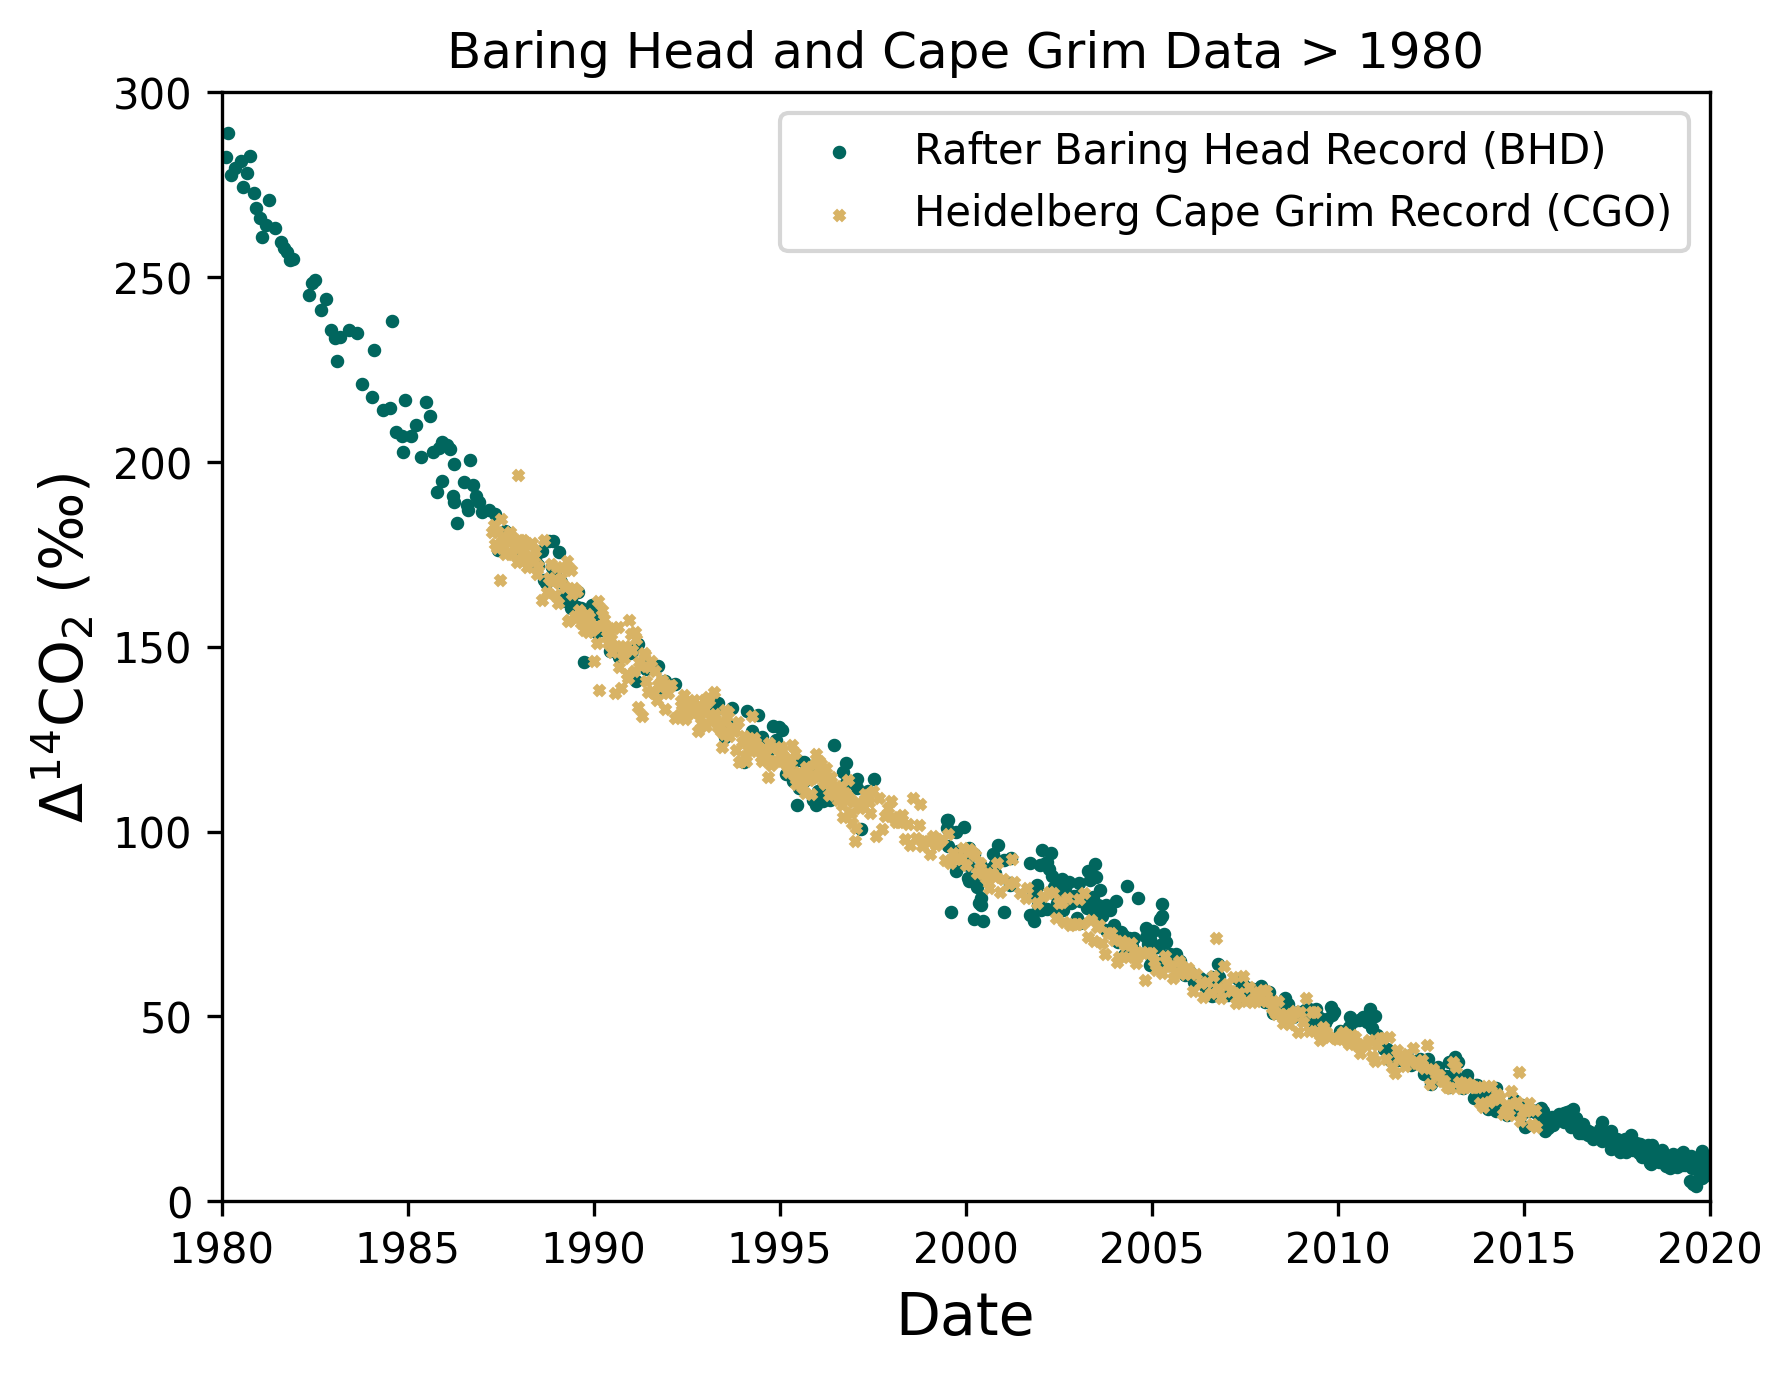
\includegraphics[width=1\textwidth]{/mnt/c/Users/clewis/IdeaProjects/GNS/Interlab_Comparison/output/DEV_FirstDraft_figure1.png}
  \caption{Vizualization of the Monte Carlo simulation to generate an uncertainty estimate about the CCGCRV curve smoothing algoritm. }
  \label{fig:montecarloexplained}
\end{figure}